\documentclass{exam}
\providecommand{\abs}[1]{\lvert#1\rvert}
\providecommand{\norm}[1]{\lVert#1\rVert}
\usepackage[utf8]{inputenc}
\usepackage[spanish, es-nolayout]{babel}		
\usepackage{amsmath}						
\usepackage{amsthm}							
\usepackage{amssymb}						
\usepackage{graphicx} 					
\usepackage{float}						
\usepackage{verbatim}					
\usepackage{url}								
\usepackage{subfig}				 
\usepackage{psfrag}			
\usepackage{multicol}
\usepackage{multirow}
\usepackage[bottom]{footmisc}
\usepackage{bigstrut}
\usepackage{color}
	\definecolor{ceruleanblue}{rgb}{0.16, 0.32, 0.75}
	\definecolor{coolblack}{rgb}{0.0, 0.18, 0.39}
	\definecolor{darkgreen}{rgb}{0.0, 0.2, 0.13}
\usepackage{multirow,hhline}
\usepackage{hyperref}
\hypersetup{
    colorlinks=true,
    linkcolor=black, % Color del enlace interno (por ejemplo, índice)
    urlcolor=black, % Color de los enlaces URL
    citecolor=black, % Color de las citas
}
\usepackage{tikz}
\renewcommand{\thefootnote}{\fnsymbol{footnote}}


\pagestyle{headandfoot}					
\headrule 										

\firstpageheader{
\includegraphics[scale=0.2]{Imágenes/Logo2.png}}{}{\scriptsize{Departamento de Economía} \\ \scriptsize{Facultad de Economía y Negocios}}
\runningheader{\scriptsize{
\includegraphics[scale=0.2]{Imágenes/Logo2.png}}}{\scriptsize Microeconomía II \\ \scriptsize{Otoño 2024}} {\scriptsize{Departamento de Economía} \\ \scriptsize{Facultad de Economía y Negocios}}

\footrule
\footer{}{\scriptsize{P\'agina \thepage\ de \numpages}}{}
\parindent = 0pt
\renewcommand\partlabel{(\thepartno.)}
\renewcommand\thesubpart{\roman{subpart}}


\printanswers  
\renewcommand{\solutiontitle}{\noindent\textbf{Respuesta:}\par\noindent\sffamily}

\begin{document}
\begin{center}

\LARGE{\textbf{Microeconomía II}}

\medskip
\normalsize \textbf{Profesora:} Paola Bordón

\normalsize \textbf{Ayudantes:} Ayelén Sandoval \& Joaquín Martínez\footnote[2]{joamartine@fen.uchile.cl}


\medskip
\large{\textbf{Ayudantía 8 - Diferenciación y Discriminación}}

\end{center}

\tableofcontents

\renewcommand{\thefootnote}{\Roman{footnote}}

\section{Comentes}
\subsection{Discriminación de precios}

\begin{itemize}
    \item[\textbf{a.}] ¿Cuál es la diferencia entre discriminación de primer y tercer grado?
    \begin{solution}
        En la discriminación de primer grado la firma puede fijar el precio que maximice su excedente dejando nada del excedente al consumidor, conocido como precio de reserva.

        En la discriminación de tercer grado la firma explota las características observables del comprador para cobrar precios diferenciados según el grupo. 
    \end{solution}
    \item[\textbf{b.}] Caracterice los mercados en los que suele haber discriminación de primer grado y tercer grado. 
    \begin{solution}
        En los mercados en donde suele haber discriminación de primer grados son:
        \begin{itemize}
            \item Mercados donde el número de compradores (“customers”) es relativamente pequeño y el vendedor posee considerable información sobre los compradores.
            \item Industrias: concreto fresco, aviones de pasajeros, software especializada para empresas, etc.
            \item A pesar que existe un precio de lista, cada cliente recibe un descuento que se negocia. Precio final de depende de la disposición a pagar del cliente y su poder de negociación.
        \end{itemize}
        Por otro lado los mercados donde suele haber discriminación de tercer grado son mercados más grandes donde los costos de información son mayores, por ejemplo los pasajes del transporte público. 
    \end{solution}
    \item[\textbf{c.}] Es imposible que una firma monopólica logre captar todo el excedente del consumidor, puesto que los precios y la estrategia que impongan dependerán también de factores como la elasticidad de la demanda.
    \begin{solution}
        Es verdad que en la práctica es difícil que se logre captar todo el excedente, pero si el monopolio tiene información perfecta sobre la disposición a pagar de los consumidores podría imponer una estrategia de discriminación de precios en primer grado, donde cada individuo paga el máximo que está dispuesto por el producto en cuestión, generando que el excedente sea nulo para los consumidores y la firma se lleve todo el excedente del mercado.
    \end{solution}
    \item[\textbf{d.}] ¿Discriminar o no discriminar? Discuta los principios básicos para responder esta pregunta.
    \begin{solution}
    Cualquier baja en la producción suele llevar a que el \textbf{bienestar total} baje. Discriminación que aumenta la demanda del producto/servicio suele aumentar el bienestar (TNE por ejemplo), no hay consumidor más triste como el que no consume. 
        \begin{itemize}
            \item Si la producción total cae con la discriminación, el bienestar total disminuye.
            \item Si un monopolista que no discrimina cierra un mercado, es mejor discriminar.
        \end{itemize}
    \end{solution}
    \end{itemize}
    \subsection{Diferenciación de producto}
    \begin{itemize}
    \item[\textbf{a.}] ¿Cuál es la diferencia entre una diferenciación horizontal y vertical?
    \begin{solution}
        Una diferenciación horizontal refiere a caracterizarse por medio de características de un mismo producto que no afecten a la calidad. Esto puede ser estética (autos), sabor (cereales), aroma (perfume), y suele ser ejemplificado como la ubicación de venta del producto.

        Por otro lado una diferenciación vertical hace referencia a un espectro de calidad de un mismo producto. Incluso no teniendo diferentes costos de producción las firmas decidirán hacer productos de distinta calidad para disminuir la competencia.

        Al fin y al cabo ambas suelen tener un mismo resultado, las empresas prefieren diferenciarse para relajar la competencia.
    \end{solution}
    \item[\textbf{b.}] Al diferenciarse horizontalmente el producto nunca cambia.
    \begin{solution}
        Falso. Hay diferenciaciones horizontales que cambian características del producto. 

        Si alguien está en búsqueda de un auto coupé deportivo de alta gama puede encontrarse con un Porsche 911 Carrera o bien con un Chevrolet Corvette Stingray. Mientras un Porsche tiene un diseño más clásico, el Chevrolet tiene un diseño más audaz. 

        Ambos tienen un precio y calidad similar, pero se diferencian en su posicionamiento frente al potencial comprador.
    \end{solution}
    \item[\textbf{c.}] El modelo de Salop es lo mismo que el modelo de Hotelling pero asumiendo una ciudad circular.
    \begin{solution}
        Falso. El modelo de Salop tiene como objetivo entender la entrada de firmas. Se supone una ciudad circular para dar por sentado que no hay ubicaciones privilegiadas sobre otras, todas las empresas son equidistantes entre sí. 
        \begin{center}
            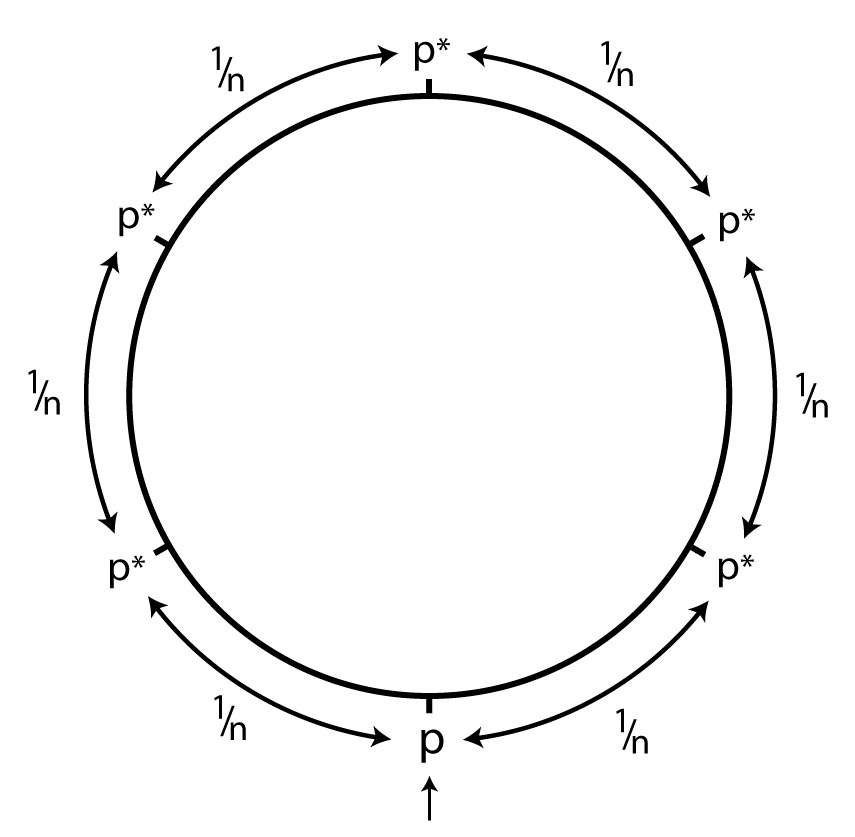
\includegraphics[width = 5.5cm]{Ayudantías ENMIC355/A8/Ciudad-circular-de-Salop.jpg}
        \end{center}
    \end{solution}
    \item[\textbf{d.}] En un modelo tipo Hotelling con decisiones de localización y luego competencia en precios, ¿Cuáles son las razones a favor y en contra de que las firmas produzcan bienes cada vez más diferenciados?
    \begin{solution}
        El efecto de demanda crea incentivos para que las firmas produzcan bienes con poca diferenciación. Cuando las empresas se acercan hacia el centro de la ciudad capturan mayor demanda.
        
        Sin embargo, el efecto estratégico nos dice que la competencia en precios en más fuerte cuanto menos diferenciados sean los bienes. Cuando las empresas se alejan del centro de la ciudad reducen la competencia por precios. 
    \end{solution}
\end{itemize}

\section{Discriminación de tercer grado}

En un pueblo del sur de Chile hay un único museo recibe a visitantes nacionales y extranjeros, quienes presentan una mayor valoración del museo. El costo marginal de producción del museo es 1 por cada visitante y no hay costos fijos. Las demandas de extranjeros y nacionales será,
\begin{align*}
    Q_E = 10-P_E \\
    Q_N = 8 - P_N
\end{align*}

\begin{itemize}
    \item[\textbf{a.}] Suponga uqe el museo monopólico fija un precio uniforme, ¿Qué precio cobra y qué beneficio obtiene? ¿Qué condición debe cumplirse para que se venda a ambos grupos?
    \begin{solution}
        La firma maximiza beneficios sobre la demanda agregada,
        \begin{equation*}
            Q_T = 18-2P
        \end{equation*}
        El museo resuelve,
        \begin{align*}
            \max_{P} & \quad \Pi = (P-c)(18-2P) \\
            \textbf{CPO:} & \\
            \frac{\partial \Pi}{\partial P} & = 18-4P + 2c = 0 \\
            P_U &= 5
        \end{align*}
        Por lo que los beneficios serán:
        \begin{align*}
            \Pi = (5-1)(18-2\cdot 5) = 32
        \end{align*}
        Para que se les venda a ambos grupos hemos de encontrar la condición de participación. La condición de restricción a la participación la encontramos evaluando a qué precio el grupo de menor valoración no consumiría. Como las demanda del grupo de nacionales, los cuales con precios mayores a 8 no demandarían ninguna entrada. 
    \end{solution}
    \item[\textbf{b.}] Suponga ahora que el monopolio puede discriminar en tercer grado. Calcule los precios de cada mercado y los beneficios del museo.
    \begin{solution}
        Para los extranjeros el museo resuelve este problema,
        \begin{align*}
            \max_{P_{E}} \quad & \pi_E = (P_E-c)(10-P_E) \\
            & \frac{\partial  \pi_E}{\partial P_E} = 10 - 2P_E + c = 0 \\
            & P_E = \frac{10+c}{2} = 5,5
        \end{align*}
        Los beneficios del museo cobrando a los extranjeros son, 
        \begin{align*}
            \pi_E = (5,5-1)(10-5,5) = 20,25
        \end{align*}
        El museo resuelve de la misma manera sobre la demanda de los nacionales,
        \begin{align*}
            \max_{P_N} \quad & \pi_N = (P_N-c)(8-P_N) \\
            & \frac{\partial \pi_N}{\partial P_N} = 8-2P_N + c = 0 \\
            & P_N = \frac{8+c}{2} = 4,5
        \end{align*}
        Los beneficios del museo cobrándole a los nacionales será,
        \begin{align*}
            \pi_N = (4,5-1)(8-4,5) = 12,25
        \end{align*}
        Los beneficios totales serán,
        \begin{align*}
            \Pi = \pi_N + \pi_E = 32,5
        \end{align*}
    \end{solution}
    \item[\textbf{c.}] Un compañero le menciona que el museo debería enfocarse solo en el grupo de alta valoración. Demuéstrele al compañero que al museo no le conviene enfocarse solo en una parte del mercado, cuando tiene la opción de discriminar precios. 
    \begin{solution}
        Si el museo solo se enfocará en los extranjeros fijaría un precio en que solo los extranjeros demanden una cantidad positiva ($P = 8$). Los beneficios serían entonces,
        \begin{equation*}
            \pi_E = (8-1)(10-8) = 14
        \end{equation*}
        Lo cuál es bastante menor que al no discriminar o discriminar a un tercer grado. 
    \end{solution}
    \item[\textbf{d.}] Comparando los beneficios del monopolio con la estrategia de precio uniforme y de discriminación ¿Cuál le conviene más? Además, calcule los excedentes de los consumidores extranjeros y nacionales ¿Cuál grupo se beneficia de la discriminación de tercer y cuál se perjudica?
    \begin{solution}
        Anteriormente obtuvimos que al discriminar la firma tiene un aumento marginal en los beneficios, está mejor discriminando en tercer grado. 

        Para calcular el excedente de los consumidores comparamos las situaciones con precio uniforme y precio diferenciado para cada tipo de consumidor. 

        Para extranjeros el excedente en cada situación será:
        \begin{align*}
            EC^U_E &= \frac{5(10-5)}{2} = 12,5 \\
            EC^D_E &= \frac{4,5 (10-5,5)}{2} = 10,125
        \end{align*}
        Para los nacionales se tiene,
        \begin{align*}
            EC^U_N &= \frac{3(8-5)}{2} = 4,5 \\
            EC^D_N &= \frac{3,5(8-4,5)}{2} = 6,125
        \end{align*}
        El grupo de mayor valoración sale perjudicado mientras que el de menor valoración está mejor siendo discriminado. En cuanto a excedente total los consumidores están peor con discriminación. 
    \end{solution}
    \item[\textbf{e.}] ¿Qué pasa con el beneficio social? Calcule también el producto total ofrecido en cada estrategia y comente su relación con los cambios en bienestar o ineficiencias que puedan estar ocurriendo. ¿Qué otros factores explican los cambios en bienestar al pasar de una estrategia a otra?
    \begin{solution}
        El beneficio social para cada estrategia corresponda a:
        \begin{align*}
            ES^U &= \Pi^U + EC^U = 32+17 =49 \\
            ES^D &= \Pi^D + EC^D = 32,5 +16,25 = 48,75
        \end{align*}
        Se concluye que en este caso el bienestar social no aumenta con la discriminación de precios. La producción total de cada estrategia es:
        \begin{align*}
            Q^U &= 18-2P = 8 \\
            Q^D &= Q_E^D + Q_N^D = (10-5,5) + (8-4,5) = 4,5 +3,5 = 8
        \end{align*}
    \end{solution}
\end{itemize}

\section{Modelo de Hotelling}
Considere una ciudad lineal que va de $0$ a $1$, dos empresas $L$ y $R$ deciden en que parte ubicarse, $\delta _L,\delta_R \in [0,1]$. Ambas ofrecen un productos homogéneos (son sustituibles) y se ofrecen a un precio $p_L, p_R$ según cada firma.\footnote{Lo único diferente de ambos productos son el lugar de la ciudad en que se venden.} Los potenciales consumidores de estas firmas se distribuyen de forma uniforme y los caracteriza la siguiente función de utilidad,
\begin{equation*}
    U_{ij} = \bar{u} + (y-p_j) - \theta (\delta_j - v_i)^2 \label{función utilidad}
\end{equation*}
\begin{enumerate}
    \item[\textbf{a.}] Explique cada parte de la función de utilidad y su interpretación intuitiva.
    \begin{solution}
        La función de utilidad es con respecto al individuo $i$ compradno a la firma $j$. En primer lugar $\bar{u}$ es una utilidad fija que les brinda el producto, $y-p_j$ es la utilidad neta de comprar el producto a la firma $j$. 

        Por último, $\theta(\delta_j - v_i)^2$ es el costo de transporte que incurre el individuo $i$ para comprarle a la firma $j$. 
    \end{solution}
    \item[\textbf{b.}] Cuántos individuos indiferentes hay en una ciudad lineal. Qué caracteriza a estos individuos. Encuentre su ubicación. 
    \begin{solution}
        En una ciudad lineal habrá un único individuo indiferente entre comprar a la firma $L$ o $R$. Este individuo es tal que $U_{\bar{i}L} = U_{\bar{i}R}$. Su ubicación la podemos encontrar planteando tal ecuación:
        \begin{align*}
    U_{iL} &= U_{iR} \\ 
    \bar{u} + (y-p_L) - \theta (\delta_L - \bar{v})^2 &= \bar{u} + (y-p_R) - \theta (\delta_R - \bar{v})^2 \\
    (p_R - p_L) - \theta (\delta _L ^2 - 2\delta_L \bar{v} + \bar{v}^2) &= - \theta (\delta_R^2-2\delta_R \var{v} + \bar{v}^2 ) \\
    (p_R - p_L) - \theta \delta_L^2 + \theta \delta_R^2 &= 2\theta \delta _R\bar{v} - 2\theta \delta_L \bar{v}  \\
    (p_R - p_L) + \theta (\delta_R^2 - \delta_L^2 ) &= \bar{v} \cdot 2\theta (\delta _R - \delta_L) \\
    \quad \\
    \bar{v} = \frac{p_R-p_L}{2\theta (\delta_R-\delta_L)} + \frac{\delta_R^2 -\delta _L^2}{2(\delta_R-\delta_L)} \\
    \xrightarrow{(a-b)(a+b)= a^2 - b^2} \frac{p_R-p_L}{2\theta (\delta_R-\delta_L)} + \frac{\delta_R + \delta_L}{2} \\ \quad \\
    \Aboxed{\bar{v} = \frac{p_R-p_L}{2\theta (\delta_R-\delta_L)} &+ \frac{\delta_R + \delta_L}{2}}
    \end{align*}
    \end{solution}
    \item[\textbf{c.}] Calcule las cuotas de mercado de ambas firmas. 
    \begin{solution}
        La cuota de mercado de la firma $L$ serán todos los individuos a la izquierda de $\bar{v}$ y $R$ se queda con el resto del mercado $1-\bar{v}$.

\begin{align*}
    D_L(p,\delta;\theta) &= \bar{v} = \frac{p_R-p_L}{2\theta (\delta_R-\delta_L)} + \frac{\delta_R + \delta_L}{2} \\
    D_R(p,\delta;\theta) &= 1 - \bar{v} = 1 -  \frac{p_R-p_L}{2\theta (\delta_R-\delta_L)} - \frac{\delta_R + \delta_L}{2} 
\end{align*}
    \end{solution}
    En el modelo de Hotelling las firmas en un primer turno eligen donde ubicarse en la ciudad para luego en un segundo empezar a vender a un cierto precio. 
    \item[\textbf{d.}] Suponga que bajo un nuevo marco legal el precio del producto está fijado. ¿Donde les conviene ubicarse las firmas?
    \begin{solution}
        Dado que las firmas están obligadas a poner un nuevo precio, dada la ubicación de la competencia la mejor respuesta siempre será estar un $\varepsilon$ más cerca del centro ($0,5$). El equilibrio será $\delta_R = \delta_L = 0,5$.

        Aquí estamos frente a un caso de mínima diferenciación. Como los precios están dados las firmas intentarán maximizar su cuota de mercado mediante su ubicación. 

        Puede ver que si $p_R = p_L $ y $\delta_R = \delta_L = 0,5$ en las funciones de demanda $D_L(p,\delta;\theta),D_R(p,\delta;\theta)$ la demanda de cada una es $0,5$, se reparten el mercado en partes iguales.
    \end{solution}
    \item[\textbf{e.}] Ahora volvamos al escenario sin el marco regulatorio, las firmas eligen sus precios. Encuentre las funciones de reacción de ambas firmas. Encuentre el equilibrio de Nash.
    \begin{solution}
        Hacemos un cambio de variable para hacer la matemática más fácil.
\begin{align*}
    \theta(\delta_R-\delta_L) = t \\
    \frac{\delta_R+\delta_L}{2} = \tau
\end{align*}
Para la empresa $L$.
\begin{align*}
    \max_{p_L} \quad \Pi_L &= (p_L - c) \left( 
 \frac{p_R-p_L+2\tau t}{2t}  \right) \\
    & = \frac{p_Lp_R - p_L^2 +2\tau tp_L}{2t} + \frac{p_Lc-p_Rc-2\tau t c}{2t} \\
    \frac{\partial \Pi_L}{\partial p_L} & = \frac{p_R-2p_L+2\tau t +c}{2t} = 0 \\
    & = p_R -2p_L+2\tau t +c = 0 \\
    & \quad \\
    & \Aboxed{p_L = \frac{1}{2} (p_R + c) + \tau t}
\end{align*}

Para la empresa $R$.
\begin{align*}
    \max_{p_R} \quad \Pi_R &= (p_R-c) \left( \frac{p_L-p_R +2t -2t\tau}{2t}   \right) \\
    & = \frac{p_Rp_L - p_R^2 +2tp_R-2t\tau p_R}{2t} - c \frac{p_L-p_R +2t -2t\tau}{2t} \\
    \frac{\partial \Pi_R}{\partial p_R} & = p_L -2p_R+2t-2t\tau +c = 0 \\
    & \Aboxed{p_R = \frac{1}{2}(p_L + c) + t(1-\tau)}
\end{align*}

Reemplazando las simplificaciones que hicimos tendríamos esta función de reacción para la firma $L$.
\begin{align*}
    p_L^* = \frac{1}{2}(p_R+c) + \frac{\theta(\delta_R^2 -\delta_L^2)}{2}
\end{align*}
Siempre que las firmas estén a una misma distancia del centro $p_L = p_R$, por lo que podemos reemplazar para obtener el equilibrio de nash. 
\begin{equation*}
    p = c + \theta(\delta_R - \delta_L)
\end{equation*}
    \end{solution}
    \item[\textbf{f.}] Grafique las funciones de reacción. Muestre como se mueven las curvas al cambiar los costos de transporte.  
    \begin{solution}
        \textbf{ \href{https://www.geogebra.org/calculator/bv9nzjae}{\underline{Link}}}
    \end{solution}
    \item[\textbf{g.}] Supongamos que usted es un planificador social omnipotente que busca maximizar el bienestar de los consumidores. Cómo cree que debiesen ubicarse las firmas.
    \begin{solution}
        La solución socialmente óptima es la que minimiza los costes de transporte y sería $\delta_L=1/4$ y $\delta_R=3/4$. Por tanto desde el punto de vista social hay demasiada diferenciación del producto cuando el mercado es privado.
    \end{solution}
\end{enumerate}




\end{document}